\documentclass[12pt]{article}

\usepackage[utf8]{inputenc}
\usepackage[russian]{babel}
\usepackage{graphicx}
\usepackage{indentfirst}
\usepackage{booktabs}


\graphicspath{{pic/}}

\begin{document}

\begin{center}
	\LARGE 
	\textbf{Практическое занятие 1}\\
	ОСНОВЫ РАБОТЫ С MATLAB\\
\end{center}

\begin{flushright}
	\large
	Игнашов Иван\\
	Вариант 8\\
\end{flushright}



\newpage

 \section*{1. Цель работы}
Изучение интерфейса пользователя системы MATLAB и основ работы с системой в режиме прямых вычислений.
\subsection*{Порядок работы:}
\begin{itemize}
	\item В командном окне задать значения переменных, согласно варианту задания\\
	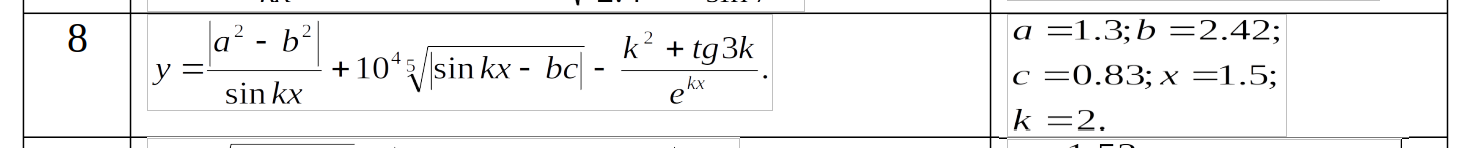
\includegraphics[width=\linewidth]{formula.png}
	
	\item Записать выражение на языке MATLAB
\end{itemize}


 \section*{2. Пример расчета и вывода данных}%
 
\begin{figure}[!h]
	\centering
	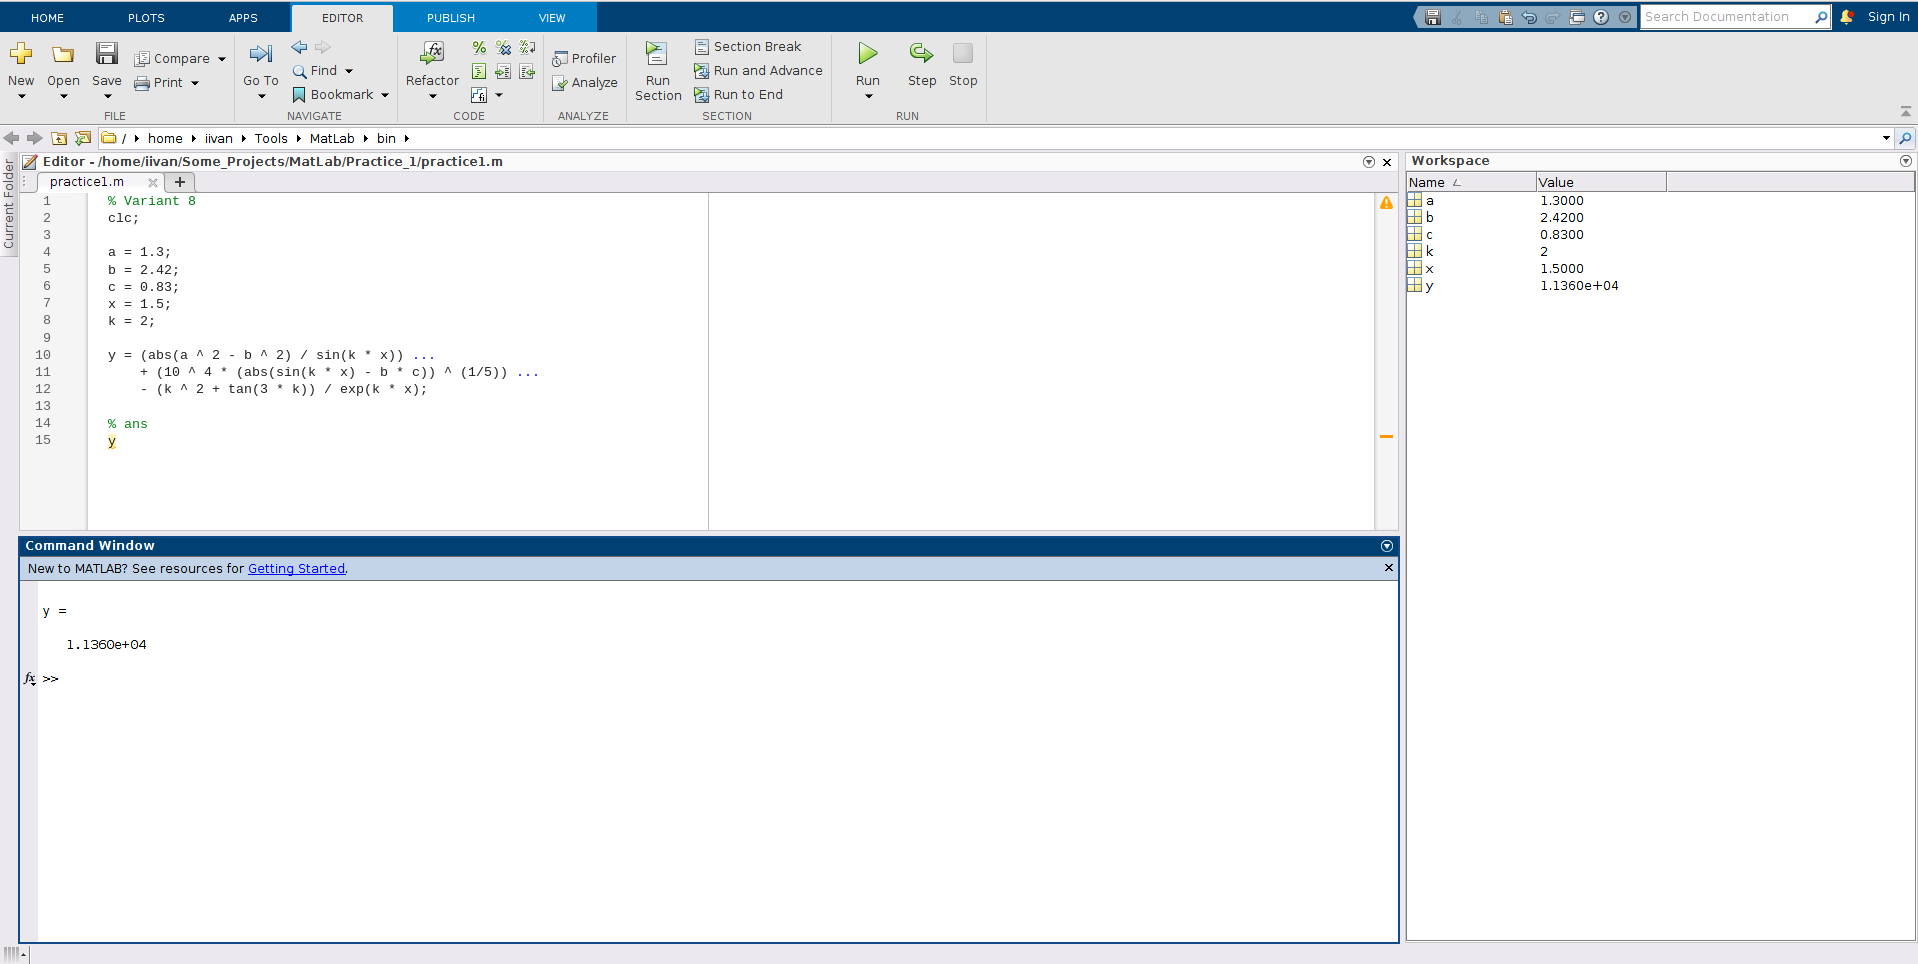
\includegraphics[width=0.75\linewidth]{full.png}
	\caption{Полный интерфейс приложения}
\end{figure}

\begin{figure}[!h]
	\centering
	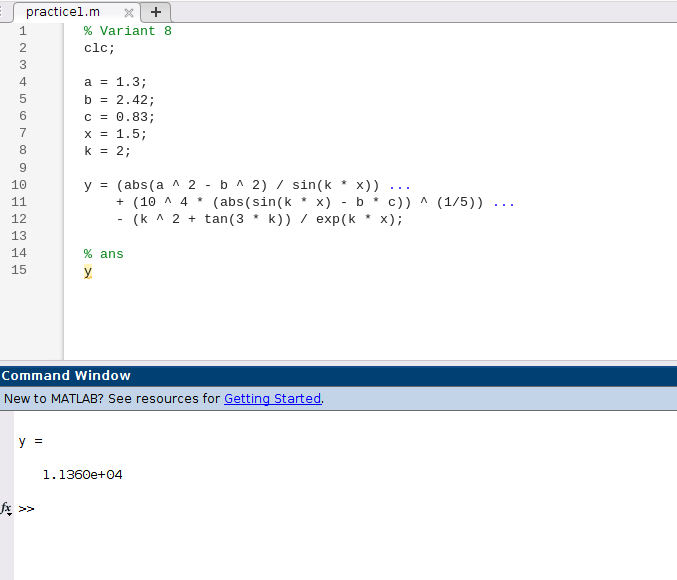
\includegraphics[width=0.75\linewidth]{calculation.png}
	\caption{Часть с расчётами и командной строкой}
\end{figure}

\begin{figure}[!h]
	\centering
	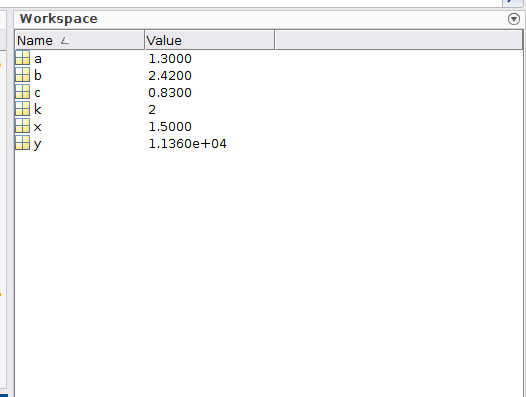
\includegraphics[width=0.5\linewidth]{workspace.png}
	\caption{Workspace с записанными данными}
\end{figure}
 

\end{document}